\UseRawInputEncoding
\documentclass[class=article,crop=false]{standalone}
\usepackage{pacco}
\begin{document}
\section{Monte-Carlo integration}
We are interested in evaluating 
\begin{equation*}
    \mu_f := \mathbb{E}_{\pi}  [f(X)] = \int_S f(x) \pi(dx)
\end{equation*}
as an integration problem.
If $S$ is discrete this takes a more familiar form $\sum_{i \in S}f(i)\pi_i$ \\
The problems can arise from the fact that$\pi$ can be multidimensional, and possibly unmormalized. Some example of these situations may be:
\begin{itemize}
    \item $f(x) = 1$ $\implies \mu_f$ is normalizing constant.
    \item If $f$ is the identity we are calculating the mean of $\pi$.
    \item If $f(x) = \mathbbm{1}_A(x) $ then tail probability and confidence intervals. 
\end{itemize}
We can also be interested in finding 
\begin{equation*}
    argmax_{x \in S} \pi (x) 
\end{equation*}
and this is an optimization problem, like for instance the mode of a distribution of interest. \\
Often an analytical computation is unfeasible and thus we need to use an approximation. Deterministic approximation include:
\begin{itemize}
    \item Riemann integration: given a partition of $S$ through points  $x_1, \dots, x_n$ then 
    \begin{equation*}
        \sum_{i=1}^n f(x_i) \pi (x_i) (x_i+x_{i-1}) \rightarrow \int f d\pi
    \end{equation*}
    as $sup_i |x_i+x_{i-1}| \rightarrow 0$.picture \\
    potentially ineficient especially in high dimention.
    \item Laplace approximation: use a Gaussian kernel to approximate a function of interest centered at the mode.
    \end{itemize}
    \begin{example}
       Let $f$ be unimodal:
    \begin{equation*}
        \int f (x) dx = \int e^{h(x)} dx 
    \end{equation*}
    take $h(x)= log f(x)$ and take a taylor of $h$ around the mode of $f$
    \begin{equation*}
        h(x)  \approx h (x_0) + \underbrace{h'(x_0)(x-x0)}_{f'/f|_{x_0}=0}+ 1/2h''(x_0)(x-x0) manca 
    \end{equation*}
    negative because we are at the mode
    \begin{equation*}
        \int f(x) dx \approx e ^{h(x_0)} \int  e ^{1/2 |h''(x_0)|(x-x0)} dx=
    \end{equation*}
    multiply and divide by $c:=\sqrt{2 \pi |h''(x_0)|^{-1}}$ and we have 
    \begin{equation*}
        =f(x_0) c \int \mathcal{N}(x; x_0, |h''(x_0)|^{-1})dx
    \end{equation*}
    this approximation is only good around the mode, but it loses a great part of its accuracy when we depart from the centre of the distribution: this makes it particularly bad for approximating, for instance, tails of a distribution. Moreover, if we work in high dimension more problems arise. $f$ needs to be unimodal, else this approach can fail (e.g. mixture models that came up a lot in statistics)     
    \end{example}

Deterministic approximations typically do not exploit information about the shape of the distribution of interest and this naturally leads to \enf{stochastic approximation}. 
\subsection{The Monte Carlo principle}
the main idea consists in exploiting information about $\pi$ and concentrate resources where they are most useful. From a general point of view simulate from $\pi$ and compute an approximation of the functional of interest. 

\begin{algorithm}{\enf{General strategy:}}
\begin{itemize}
    \item sample $X_1, \dots, X_n \stackrel{iid}{\sim}\pi$. \\
    ($N=$ MC sample size )
    \item $\mu_N = \frac{1}{N} \sum_{i=1}^N f(X_i) $\\
    \end{itemize}
    \end{algorithm}
    Note that if $\pi_N:= \frac{1}{N} \sum_{i=1}^N \delta_{X_i}$ then we have just 
    \begin{equation*}
        \mu_N = \int f(x) \pi_N (dx) = \frac{1}{N} \sum_{i=1}^N\int f(x)\delta_{X_i}  (dx) = \frac{1}{N} \sum_{i=1}^N f(X_i)
    \end{equation*}
    now 
    \[
    \mathbb{E}_\pi\left[\mu_N\right]=\frac{1}{N}\sum_{i=1}^{N}\mathbb{E}_\pi\left[f(x_i)\right]=\int f(x)\pi(dx)=\mu_f
    \]
    so $\mu_N$ is unbiased. Moreover, if $\mathbb{E}_\pi(f)<\infty$,
    \[
    \mu_N\xrightarrow{a.s.}\mu_f\qquad\text{by SLLN.}
    \]
    If $\mathbb{E}_{\pi} (f^2) < \infty$, set 
    \begin{equation*}
        \sigma_f ^2 := Var [f(X)] = \mathbb{E}_{\pi} [(f(X)- \mu_f)^2]
    \end{equation*}
    then $\mu_N$ has variance 
    \begin{equation*}
         \sigma_N ^2= Var(\mu_N) = \frac{\sigma_f ^2}{N}
    \end{equation*}
    so $\mu_N$ is a constant estimator of $\mu_f$. We also have a central limit theorem
    \begin{equation*}
         \sqrt{N} (\mu_N-\mu_f) \xrightarrow{d} \mathcal{N}(0, \sigma_f ^2)
    \end{equation*}
    to be used, e.g., for constructing asymptotic confidence intervals. 
Some potential issues are:
\begin{itemize}
    \item it may be computationally expensive;
    \item sampling directly from $\pi$ could be unfeasible and/or too difficult (e.g. high-dimensional distribution, distributions whose normalizing constant is unknown...).
\end{itemize}
    example. $Z \in \mathcal{N}(0,1)$. We are interested in 
    \begin{equation*}
        \mu= \mathbb{P}(Z> 5) = \int _{\mathbb{R}}\underbrace{\mathbbm{1}(x >5)}_{\mathclap{f(x)}} \varphi (z) dz
    \end{equation*}
    The value for $\mu$ is around $2.87\times10^{-7}$. Now draw $X_i \stackrel{i.i.d.}{\sim} \mathcal{N}(0,1)$
    \begin{equation*}
        \mu_N = \frac{1}{N} \sum_{i=1}^N \mathbbm{1}(x_i >5) \rightarrow \mu
    \end{equation*}
    This means that as long as we draw $N<\mathcal{O}(10^7)$ we expect to see a positive indicator... 0 times. This is an example of situation where simulating $\pi$ is computationally infeasible. To face this limitation, we turn to a very important idea: the \textbf{rejection sampling}. 
\subsection{Rejection Sampling}
\begin{algorithm}
    until $N$ points are saved repeat:
    \begin{itemize}
        \item draw independently $Z \sim Unif (a,b)$ and $ Y \sim Unif(0,M) $;
        \item if $y \leq \pi(z)$, set $X=z$.
    \end{itemize}
\end{algorithm}
\begin{figure}[H]
\centering
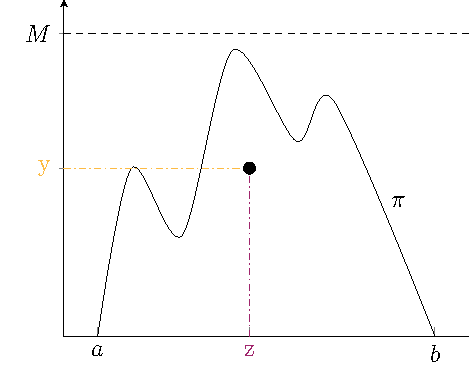
\includegraphics{../standalones/pdfs/rejection1}
    \label{rejsampl}
\end{figure}
Only points under $\pi $ are kept, and these are draws from $\pi$. Cdf of accepted points:
\begin{equation*}
\begin{split}
    \mathbb{P}(Z \leq x| Y \leq \pi(Z))&= \frac{\mathbb{P}(Z \leq x, Y \leq \pi(Z))}{\mathbb{P}( Y \leq \pi(Z))}\\
    &= \frac{\mathbb{P}(Z \leq x, Y \leq \pi(Z))}{\mathbb{P}( Z \leq b, Y \leq \pi(Z))}\\
    &= \frac{\int_a^x \int_0 ^{\pi(Z)}\frac{1}{M}dy \frac{1}{b-a}dz} {\int_a^b \int_0 ^{\pi(Z)}\frac{1}{M}dy \frac{1}{b-a}dz}\\
    &= \int_a^x \pi(Z) dz
\end{split}
\end{equation*}
so now we can compute  $\mu_N = \frac{1}{N} \sum_{i=1}^N f(X_i) $. 

If the support of $\pi$ is unbounded, we cannot draw from $Unif(a,b)$, the idea is that we are gonna use a non uniform bound and an auxiliary distribution. \\
Assume:
\begin{itemize}
    \item $\exists M>0$ and a density $q$ such that
    \begin{equation*}
        \pi (x) \leq Mq(x)
    \end{equation*}
    \item we can draw from $q$, meaning that we should choose a $q$ we can simulate relatively easily.
\end{itemize}
\begin{algorithm}
    until $N$ points are saved:
\begin{itemize}
    \item draw $Z\sim q$, with $Y|Z=z\sim Unif(0, Mq(z))$;
    \item if $Z\leqslant\pi(z)$, set $x=Z$.
\end{itemize}
\end{algorithm}
\begin{figure}[H]
\centering
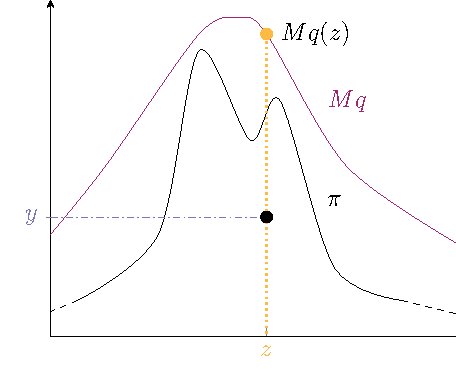
\includegraphics{../standalones/pdfs/rejection2}
    \label{res2}
\end{figure}
Verify $(-\infty\leqslant a < b \leqslant\infty)$=\[
=\dfrac{\displaystyle\int_{-\infty}^{x}\int_0^{\pi(z)}\frac{1}{\cancel{Mq(z)}}dy\,\cancel{q(z)}dz}{\displaystyle\int_{-\infty}^{\textcolor{red}{\infty}}\int_0^{\pi(z)}\frac{1}{\cancel{Mq(z)}}dy\,\cancel{q(z)}dz}=\mathbb{P}(X\leqslant x)\
\]
\begin{example}
    take $\mu=\mathbb{P}(z>5)=2.87\cdot10^{-7}$. We need a non-uniform bound:
\[
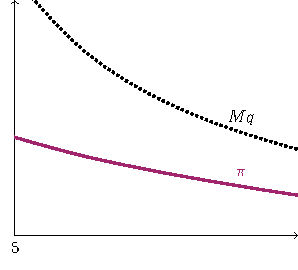
\includegraphics{../standalones/pdfs/normsampl}
\]
Choose $q(x)=e^{-(x-5)}\mathbbm{1}(x>5)$ with $M=\phi(5)$. We know that
\[\mu_N=\% \text{ of accepted points}\times\underbrace{\text{area of graph where we generate values}}_{\int_5^\infty Mq(x)dx=M\int_5^\infty e^{-(x-5)}d=M}\]
This algorithm is generally more efficient than naive Monte-Carlo where we would have to generate $x_i\sim N(0,1)$ variables and keep $x_i>5$. It can be, anyway, costly: the acceptance probability over an interval $(c,d)$ is
\begin{align*}
    \mathbb{P}(c\leqslant Z\leqslant d, Y\leqslant\pi(z))&=\int_c^d\int_0^{\pi(z)}\frac{dy}{Mq(z)}q(z)dz\\
    &=\frac{1}{M}\int_c^d\pi(z)dz.
\end{align*}
In general, over the support, the acceptance probability is $\frac{1}{N}$. So, in order to have $N$ points, we need to generate a number of points equal to
\[N'\sim Neg-Bin\Bigl(N,\frac{1}{M}\Bigr).\]
\[\frac{1}{M}\int_5^\infty\pi(x)dx=\frac{2.87\cdot10^{-7}}{1.49\cdot10^{-6}}=0.19\]
\end{example}
\subsection{Importance Sampling}
This idea starts with a little analytical trick, in general terms the idea is to use all generated samples. Unlike the accept-reject method. \\
\begin{equation*}
\begin{split}
    \mu&= \mathbb{E}_{\pi}[f(x)] = \int f(x) \pi(x) dx = \int f(x) \frac{\pi(x)}{q(x)} q(x) dx \\
    &= \mathbb{E}_{q}[f(x)\frac{\pi(x)}{q(x)}]
\end{split}
\end{equation*}
where $q$ is a density whose support include that of $\pi$.\\ (i.e. $q(x)=0$ $\implies$ $\pi(x)=0$)\\
Then we can:
\begin{itemize}
    \item draw $X_i \stackrel{\text{i.i.d.}}{\sim} q$ 
    \item assign weight $w(x_i):= \frac{\pi(X_i)}{q(X_ i)}$ to $X_i$. ($w$ importance weight)
    \item  set 
    \begin{equation*}
        \mu_N= \frac{1}{N} \sum_{i=1}^N f(X_i)w(X_i)
    \end{equation*}
\end{itemize}
Then
\begin{equation*}
    \mathbb{E}_q[\mu_N]= \mathbb{E}_q [f(x)w(x)] \stackrel{above}{=} \mu 
\end{equation*}
moreover
\begin{equation*}
    \mu_N \xrightarrow{a.s.} \mu \hspace{0.5 cm} \text{ as } n \rightarrow + \infty
\end{equation*}
\begin{figure}[H]
    \centering
    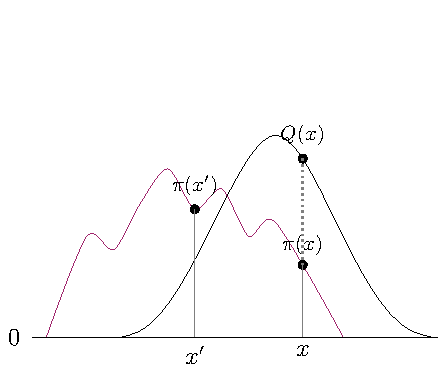
\includegraphics{../standalones/pdfs/impsamp}
    \label{impsamp}
\end{figure}
\begin{itemize}
    \item down-weight importance of $x$\\
    $\pi (x) < q(x) \implies w(x) = \frac{\pi (x)}{q(x)}< 1$. 
    \item $w(x')>1$ up-weight of $x'$.
\end{itemize}
draws in relevant regions are up-weighed automatically and no draws are wasted. The choice of $q$ is more flexible than in the AR method.\\ 
\textbf{Toy Example.} $\mathbb{P}(Z>5) = \mu= 2.87 \times 10 ^{-7}$\\\
Use 
\begin{equation*}
    q(x)= e ^{-(x-5)} \mathbbm{1}_{\{x>5\}},
\end{equation*}
and so 
\begin{equation*}
    \mu = \int_5^{\infty} \phi(x) dx= \int_{\mathbb{R}} \mathbbm{1}_{\{x>5\}} \phi(x) dx = \int_{\mathbb{R}} \underbrace{\mathbbm{1}_{\{x>5\}}}_{= f(x)} \underbrace{\frac{\phi(x)}{q(x)}}_{=w(x)} q(x) dx
\end{equation*}
so $X_i \stackrel{\text{i.i.d.}}{\sim} q $.
\begin{equation*}
    \mu_N= \frac{1}{N} \sum_{i=1}^N f(X_i)w(X_i) = \frac{1}{N} \sum_{i=1}^N \underbrace{\mathbbm{1}_{X_i>5} }_{\text{since } X_i \sim q }\frac{\phi(x_i)}{q(x_i)}  = \frac{1}{N} \sum_{i=1}^N\frac{\phi(x_i)}{q(x_i)} 
\end{equation*}
Additional upside:\\
if $\pi= \frac{\tilde{\pi}}{z}$ with $z$ unknown. Then
\begin{equation*}
    \mu = \int f(x) \pi (x) dx = \int f(x)\frac{\tilde{\pi(x)}}{z q(x)} q(x) dx 
\end{equation*}
\begin{equation*}
    \rightarrow \ \ z= \int \tilde{\pi(x)} dx = \int \frac{\tilde{\pi(x)}}{q(x)}q(x) dx 
\end{equation*}
so setting $\tilde{w}(x)=\frac{\tilde{\pi(x)}}{q(x)}$ we have 
\begin{equation*}
     \mu = \underbrace{\frac{\int f(x) \Tilde{w}(x) q(x) dx }{\int \Tilde{w}(x) q(x) dx}}_{\text{self-normalizing estimate}}
\end{equation*}
Hence for $X_i \stackrel{\text{i.i.d.}}{\sim} q $ we now have 
\begin{equation*}
    \Tilde{\mu}_N = \frac{\frac{1}{N} \sum_{i=1}^N f(X_i)\Tilde{w}(X_i)}{\frac{1}{N} \sum_{j=1}^N \Tilde{w}(X_j)} = \sum_{i=1}^N  f(X_i) \hat{w}(X_i)
\end{equation*}
with $\hat{w}(X_i)= \frac{\Tilde{w}(X_i)}{\sum_{j=1}^N \Tilde{w}(X_j)}$. Strong law of large numbers still applies. \\
\subsection{Markov-Chain Monte-Carlo}
When:
\begin{itemize}
    \item Tails of $q$ versus $\pi$ can be very different so that $w(x)$ possibly unbounded
    \item $q$ may be difficult to identify in high-dimensions
\end{itemize}
Idea: we can generate draws from $\pi$ using Markov Chains, obtaining what is called \textbf{Markov Chains Monte Carlo}.\\
Given a target distribution $\pi$, we want to construct an ergodic Markov chain $X$ with stationary distribution $\pi$, and use its trajectory to get draws from $\pi$. \\
Assume for now $P$ is ergodic. \\ Given an intial state $X_0$, we can in principal simulate trajectory :\\
$\forall \ n \geq 0 $, if $X_n = i$, draw $X_{n+1}=j$ with probability $p_{ij}$
from ergodicity we know 
\begin{equation*}
    \exists n_0 \in \mathbb{N}: X_n \sim \pi \ \ \forall n \geq n_0
\end{equation*}
Such $n_0$ is called Mixing time, meant as an order of magnitude, not as a step. (e.g. $n_0=O(10^4)$)\\
Studying mixing times is typically difficult. Usually one uses convergence test or diagnostics.
(there is literature, Gelman-Rubin criterion).\\
Suppose we know $n_0$. Then 
\begin{itemize}
    \item simulate $\{X_n ^{(i)}, n \leq n_0\}$ for $i=1, \dots, N$.
    \item set $Y_i = X_{n_0+i}$ (sample path endpoint).
\end{itemize}
Then $(Y_i, \dots, Y_N)$ is the MCMC sample. These are i.i.d $\sim \pi$ (assume $X_0^{(i)}$ independent).\\
$\implies$ we are back t0 the Monte-Carlo scenario with 
\begin{equation*}
    \mu_N = \frac{1}{N}\sum_{i=1}^N f(Y_i) \xrightarrow{a.s.} \mu_f
\end{equation*}
where 
\begin{equation*}
    Var(\mu_N)= \frac{\sigma_f^2}{N}, \  \  \ \sigma_f^2= Var_{\pi}(f(Y)). 
\end{equation*}
However we are discarding  $N=n_0$ sample. If, for example, $N= 10^4$, $n_0= 10^5$ $\implies 10^9$, which is expensive.\\
alternatively, we can think of using a single chain . \\
\begin{algorithm}[\textbf{Generic MCMC strategy}]
   Given $N$:
\begin{itemize}
    \item simulate $\{X_n, n\}$
    \item  for $n_0$ large enough, set 
    \begin{equation*}
        \hat{Y}_i= X_{n_0+i}, \ \ i = 1,\dots,N 
    \end{equation*}
\end{itemize}
\begin{equation*}
    \implies \mu_N = \frac{1}{N}\sum_{i=1}^N f(\hat{Y}_i)\approx \mu_f 
\end{equation*} 
\end{algorithm}

\begin{figure}[H]
    \centering
    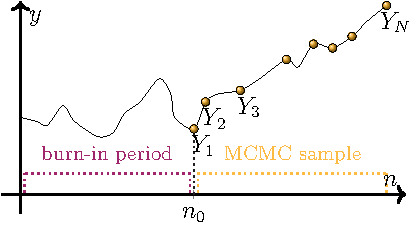
\includegraphics{../standalones/pdfs/burnin}
\label{burnin}
\end{figure}
Only $n_0$ values wasted. %it's a strong statement man. 
The MCMC samples are now correlated and the MCMC estimator is now no longer a generic sample average but it is an ergodic average. In terms of theoretical result we have the ergodic theorem that guarantees 
\begin{equation*}
    \frac{1}{N}\sum_{i=1}^N f(\hat{Y}_i) \xrightarrow{a.s.} \mu_f = \mathbb{E}_{\pi}[f(Y)]
\end{equation*}
for any initial distribution.\\ Understand what we are losing, consider the variance of $\hat{\mu}_N$ 
\begin{equation*}
    Var\Bigg(\frac{1}{N}\sum_{i=1}^N f(\hat{y}_i)\Bigg) = \frac{1}{N^2}\sum_{i=1}^N\Bigg[Var\Big(f(\hat{y}_i)\Big)+2\sum_{k=1}^{N-1}Cov\Big(\underbrace{f(\hat{y}_i,f(\hat{y}_{i+k})}_{\mathclap{\text{autocovariance function}}}\Big)\Bigg]
\end{equation*}
at equilibrium, $Var$ and $Cov$ do not depend on time but only on the lag.  In particular $Var(f(\hat{Y}_i))= \sigma_f^2$. 
\begin{equation*}
    %Ha ripreso la roba di prima
    \frac{1}{N^2}  \sum_{i=1}^N \left[\sigma_f^2 + 2 \sigma_f^2\underbracket{\sum_{k=1}^{N-i}\frac{Cov(f(\hat{Y}_i),f(\hat{Y}_{i+k} )}{\sigma_f^2}}_{\mathclap{\gamma_k=Corr\left(f(\hat{y}_i,f(\hat{y}_{i+k})\right)}}\right] \approx \frac{\sigma_f^2}{N}(1+\sum_{k\geq 1}\gamma_k)
\end{equation*}
This is higher the the variance of the MCMC estimator with $N$ chains (in fact it is a MC estimator). The quantity 
\begin{equation*}
    \Tilde{N} = \frac{N}{1 +2\sum_{k\geq 1}\gamma_k }
\end{equation*}
is called \textbf{effective sample size}. Indeed

\begin{align*}
       &\frac{Var(\hat{\mu}_N)}{Var(\mu_N)} = \frac{\sigma_f^2/\Tilde{N}}{\sigma_f^2/N} \\
    \implies &ESS= N \frac{Var(\hat{\mu}_N)}{Var(\mu_N)}  \in [0,N] 
\end{align*}

so the $ESS$ reppresent the size of an iid smaple with the same variance of the MCMC sample, giving a measure of the loss of efficiency determined by using a correlated sample. \\
Here we are hoping $\gamma_k$ decays fast. Other wise the common practice is to perform what is called thinning, that is setting 
\begin{equation*}
    \hat{Y}_i = X_{n_0+ih } \hspace{0.5 cm} i = 1, \dots, N
\end{equation*}
for a chosen $h \in \mathbb{N}$. This lowering the correlation among succesive samples. \\
In fact debated practice 
\begin{itemize}
    \item now we discard a higher number of samples.
    \item it is belived that keeping all sample after the burn-in yield's a better approximation of $\mu_f$.
\end{itemize}
Observation even if are correlated are pieces of information so don't waste them, on the other hand maybe you want to remove correlation. 
\subsection{Metropolis-Hastings algorithm}
The \textbf{Metropolis-Hastings algorithm} has been selected among the 10 most important algorithms of the 20th century. 

The idea consists in running a chain with arbitrary transition matrix, but sometimes suppressing transition (in a "right way"). Given a target $\pi$ on $S$, let:
\begin{itemize}
    \item [-]$Q$ be an aribtrary, irreducible transition matrix called \textit{proposal matrix};
    \item [-]$A$ be a matrix with entries $a_{ij}\in[0,1]$ called \textit{acceptance matrix}.
\end{itemize}
\begin{algorithm}[\textbf{Generic Metropolis-Hastings}]
    For $n\geqslant 1$, if $X_{n-1}=i$:
    \begin{itemize}
        \item [-] draw $j$ with probability $q_{ij}$;
        \item [-] set $X_n=j$ with probability $a_{ij}$; else set $X_n=X_{n-1}$
    \end{itemize}
\end{algorithm}
$Q$ provides proposal states: from row $i$ draw state $j$, $A$ tells us if we should go in $j$ or stay where we are. The resulting transitions are:
\[
p_{ij}=\begin{cases}
    q_{ij}a_{ij} &j\neq i\\
    1-\sum_{k\in S}  q_{ik}a_{ik} &j=i.
\end{cases}
\]
\begin{itemize}
    \item[$\rightarrow$]$Q=(q_{ij})_{i,j}\in S$ is aribtrary (which means we can choose a distribution easy to simulate from);
    \item[$\rightarrow$]$P=(p_{ij})_{i,j\in S}$ is irreducible since $Q$ is aperiodic and since $X_n=X_{n-1}$ with positive probability.
\end{itemize}
So if we show $P$ has invariant distribution $\pi$, then it is positive recurrent and the ergodic theorem applies: $\pi$ is therefore also the equilibrium distribution. \\
Idea: occasionally suppress transitions to state that are less likely "with respect to $\pi$", so to speak.
\begin{proposition}
    The Metropolis Hastings algirthm with proposal matrix $Q$ and acceptance probabilities
        \[
        a_{ij}=\min\bigg\{1,\frac{\pi_jq_{ji}}{\pi_iq_{ij}}\bigg\}
        \]
        generates a \textbf{reversible chain} with respect to $\pi$.
\end{proposition}
\begin{proof2}
    We need to show that $\pi_ip_{ij}=\pi_jp_{ji}$ (detailed balance for the resulting chain).
        \begin{align*}
            \pi_ip_{ij}&=\pi_iq_{ij}a_{ij}\\
            &=\pi_iq_{ij}\min\bigg\{1,\frac{\pi_jq_{ji}}{\pi_iq_{ij}}\bigg\}=\\
            &=min\bigg\{\pi_iq_{ij},\pi_jq_{ji}\bigg\}.
        \end{align*}
        But since minimum is symmetric and \[
        min\big\{\pi_jq_{ji},\pi_iq_{ij}\big\}=min\big\{\pi_iq_{ij},\pi_jq_{j1}\big\}.
        \]
        starting from $\pi_jq_{ji}$ yields the same term, so $\pi_i p_{ij}=\pi_jp_{ji}$.
\end{proof2}
\begin{algorithm}\enf{Metropolis-Hastings Algorithm}
     For $n\geqslant1$, if $X_{n-1}=i$:
    \begin{itemize}
        \item [-] draw $J=j$ with probability $q_{ij}$;
        \item [-] draw $U\sim Unif(0,1)$;
        \item [-] if $U<\min\left\{1,\frac{\pi_jq_{ji}}{\pi_iq_{ij}}\right\}$ set $X_n=j$; else $X_n=X_{n-1}$
    \end{itemize}
\end{algorithm}
This algorithm has important features:
\begin{itemize}
    \item the proposal distribution is fully arbitrary, with the sole condition of being irreducible. This leaves us a lot of freedom.
    \item it applies even if the normalizing constant of $pi$ is unknown, since
    \[
    \frac{\pi_j}{\pi_i}=\frac{\tilde{\pi}_j/\cancel{z}}{\tilde{\pi}_i/\cancel{z}}=\frac{\tilde{\pi}_j}{\tilde{\pi}_i}
    \]
\end{itemize}
\begin{example}
    \[
\pi(\cdot)=cPois(\cdot;\lambda_1)+(1-c)Pois(\cdot;\lambda_2)
\]
is a mixture of Poisson distributions. We want to reconstruct this target using ergodic average. Propose states with a simple MC: we will use a $B\&D\left(\frac{1}{2},\frac{1}{2}\right)$ (i.e. a symmetric random walk on $\Z_+$).
\begin{align*}
    \implies &q_{ij}=\frac{1}{2}\qquad\text{for }j=(i\pm1)^+\\
    & a_{ij}=\min\{1,\alpha_{ij}\}\qquad\alpha_{ij}=\frac{\pi_jq_{ji}}{\pi_iq_{ij}}\\
    \implies &\alpha_{ij}=\frac{cPois(j;\lambda_1)+(1-c)Pois(j;\lambda_2)}{cPois(i;\lambda_1)+(1-c)Pois(i;\lambda_2)}\cdot\frac{\cancel{1/2}}{\cancel{1/2}}
\end{align*} This last equality is true for $j=(i\pm1)^+$ and arbitrary for all other $j$s, which are not going to be proposed wince we use a random variable. The code can be found in appendix. %\ref{poiscode}.
The random walk is not positive recurrent, but Metropolis-Hastings "corrects" the trajectory so that it basically becomes recurrent.
\end{example}
The previous example refers to a typical class of Metropolis-Hastings algorithms called \textit{random walk Metropolis-Hastings}, where
\[
X_n=X_{n-1}+Z_n
\]
Where $Z_n$ has symmetric distribution around zero. The example provided, in particular, is a special case called \textbf{Metropolis} algorithm, where the proposal is symmetric so that
\[
q_{ij}=q_{ji}\implies a_{ij}=\min\left\{1,\frac{\pi_j}{\pi_i}\right\}.
\]
So:
\begin{itemize}
    \item if $\pi_j<\pi_i$ we accept the step with probability $<0$;
    \item if $\pi_j>\pi_i$ we accept the step with probability 1.
\end{itemize}

We can interpret this consequence of the algorithm as the fact that if the density of the new step increases, we accept the step and we continue exploring that direction; otherwise, we still have a chance to accept the new steps even if it leads us to a zone with lower density. Of course, if we only accepted steps that increase the density we would basically have an optimization algorithm that maximizes probability density (which is not what we want).
\begin{example}
    \[
\pi(\cdot)=cN(\cdot;\mu_1,\sigma_1^2)+(1-c)N(\cdot;\mu_2,\sigma_2^2).
\]
We can use a random walk Metropolis-Hastings that proposes
\[
Y=X+Z\qquad Z\sim N(0,\sigma_0^2)
\]
if $X_{n-1}=X$, and $\alpha_{ij}$ is now
\[
\alpha(x,y)=\frac{\pi(y)q(x|y)}{\pi(x)q(y|x)}
\]
where $q(y|x)=N(y;x,\sigma_0^2)$. They are symmetric, so
\[
\alpha(x,y)=\frac{\pi(y)}{\pi(x)}
\]
\end{example}
Another special case is the \textit{independent Metropolis-Hastings}, where the proposal does not depend on the current state, i.e.
\[
q_{ij}=q_j\implies a_{ij}=\min\left\{1,\frac{\pi_jq_i}{\pi_iq_j}\right\}=\min\left\{1,\frac{\pi_j/q_j}{\pi_i/q_i}\right\}.
\]
Proposals are accepted with probability 1 if
\[
w_j=\frac{\pi_j}{\pi_j}>\frac{\pi_i}{\pi_i}=w_i\qquad\text{(it's a reweighing)}
\]
Analogies:
\begin{itemize}
    \item with \textit{importance sampling}: $w(x)=\frac{\pi(x)}{q(x)}$ is the importance weight, i.e. we accept with probability 1 if $w_j>w_i$ (which means there has been an improvement in importance weights).
    \item with \textit{rejection sampling}: propose $z=j$ with probability $q_j$ and accept if $y\leqslant\pi_j$ where $y|z=j\sim Unif(0,Mq)$ which is the same as \[
    U<\frac{\pi_j}{Mq_j},\qquad U\sim Unif(0,1)
    \]
    that here becomes $U<\frac{\pi_j/q_j}{\pi_i/q_i}$ instead of $\frac{\pi_j}{Mq_j}$.
\end{itemize}
\subsection{Gibbs sampling}
Gibbs sampling is formally a special case of Metropolis-Hastings but it found wider applications. It is useful with:
\begin{itemize}
    \item multivariate $\pi$;
    \item models with latent variables;
    \item models specified using conditionals.
\end{itemize}
Gibbs sampling needs at least a bivariate space. Let $\pi=\pi_{X,Y}$ density on $S\times S$. We cannot sample directly from $\pi$ but we can sample from the conditionals $\pi_{X|Y}$ and $\pi_{Y|X}$.
\begin{algorithm}[\textbf{Two-component Gibbs sampler}]
    Given $(X_{n-1},Y_{n-1})=(x,y)$ as our current state,
    \begin{itemize}
        \item [-] draw $X'\sim\pi_{X|Y}(\cdot|Y)$ 
        \item [-] draw $Y'\sim\pi_{X|Y}(\cdot|X)$
        \item [-] set $(X_n,Y_n)=(X',Y')$
    \end{itemize}
\end{algorithm}
Why is this useful? If $(X,Y)\sim\pi_{x,y}$ this is equivalent to say that
\[
Y\sim \pi_y \;\text{(marginal distribution)},\quad X|Y\sim\pi_{X|Y}\;\text{(chain rule)}
\]
but if $X'\sim \pi_{X|Y}$ then 
\[
(X',Y)\sim\pi_{X,Y}
\]
which is obvious, since we drew it that way. The same holds for $Y'$, so these transitions preserve the joint distribution $\pi_{X,Y}$ which is therefore invariant.
\begin{proof2}
 The first step of the algorithm can be seen as a Metropolis-Hastings step with proposal on $S^2=S\times S$:
        \[
        q=(X',Y'|X,Y)=\pi_{X'|Y'}(X'|y)\mathbbm{1}(Y'=y).
        \]
        In practice, we fix $Y$ and then we update $X$. The acceptance rate is $\min\left\{1,\frac{\pi_jq_{ji}}{\pi_iq_{ij}}\right\}$. If we factorize in marginals and conditional we get:
        \[
        \frac{\textcolor{red}{\pi(X'Y')}\textcolor{blue}{q(X,Y|X',Y')}}{\textcolor{Dandelion}{\pi(X,Y)}\textcolor{OliveGreen}{q(X',Y'|X,Y)}}=\frac{\textcolor{red}{\pi(Y')\pi(X'|Y')}\textcolor{blue}{\pi(X|Y')\mathbbm{1}(Y=Y')}}{\textcolor{Dandelion}{\pi(Y)\pi(X|Y)}\textcolor{OliveGreen}{\pi(X'|Y)\mathbbm{1}(Y=Y')}}
        \]
        but since we imposed $Y=Y'$, all these factors cancel out:\[
        =\frac{\textcolor{red}{\cancel{\pi(Y')\pi(X'|Y')}}\textcolor{blue}{\cancel{\pi(X|Y')}\cancel{\mathbbm{1}(Y=Y')}}}{\textcolor{Dandelion}{\cancel{\pi(Y)\pi(X|Y)}}\textcolor{OliveGreen}{\cancel{\pi(X'|Y)}\cancel{\mathbbm{1}(Y=Y')}}}=1.\]
\end{proof2}
So every step of the Gibbs samples is made of 2 mini Metropolis-Hastings steps with probability of acceptance 1: we never reject any data. If we are only interested in $X$ univeriates we can sometimes augment the state space to $S\times S'$ through can auxiliary variable $Y\in S'$ paradoxally introduced to ease the computation. The transition for $X$ (marginal) can be written, integrating $Y$ out, as \[
p_X(x'|X)=\int_{S'}\pi_{Y|X}(y|x)\pi_{X|Y}(x'|y)dy.
\]
Stationarity requires, by the global balance conditions:
\[
\int_S\pi_X(x)p_X(x'|X)dx=\pi_X(x').
\]
We have
\[
\int_{S}\pi_{X}(x)p_X(x'|X)dx=\int_S\pi_X(x)\left(\int_{S'}\pi_{Y|X}(y|X)\pi_{X|Y}(x'|Y))dx\right)dy.
\]
Using Fubini's theorem
\begin{align*}
&\int_{S'} \pi_{X|Y}(x'|Y)\int_S\underbracket{\pi_{Y|X}(y|X)\pi_X(X)}_{\pi_{X,Y}(X'Y)}dxdy\\
&\int_S \underbracket{\pi_{X|Y}(x'|Y)\pi_{Y}(y)}_{\pi_{X,Y}(X',Y)}dy=\pi_X(x')
\end{align*}
A Gibbs sampler on $(X_n,Y_n)$ yields, marginally, a stationary $X_n$ chain with respect to $\pi_X$.
If we are interested in $X$, $Y$ can be sometimes an auxiliary variable: \\
\begin{itemize}
    \item we run the Gibbs sampler on $(X_n, Y_n)$
    \item discard $Y_n$
    \begin{equation*}
    \begin{split}
        \implies \ \ X_n (\text{ at stationarity })\\
        \text{is from }\pi_x = \int \pi_{X,Y}(x,y)dy
    \end{split}
    \end{equation*}
\end{itemize}
\begin{example}
    In a popular Bayesian model we have 
\begin{equation*}
    \pi_X (x) \propto x ^{\alpha+k-1} e ^{-\beta x} \frac{\Gamma(x)}{\Gamma(x+n)}, \hspace{0.5 cm } x \geqslant 0.
\end{equation*}
Normalizing and simulating from $\pi$ is not trivial, due to the presence of gamma functions. However, 
\begin{equation*}
    \frac{\Gamma(x)\Gamma(n)}{\Gamma(x+n)}=\int_0^1 y^{x-1}(1-y)^{n-1}\dif y
\end{equation*}
so we can formulate a joint model on the augmented state space $\mathbb{R}_+ \times [0,1]$.
\begin{align*}
    \pi_{X,Y}(x,y)&\propto x ^{\alpha+k-1} e ^{-\beta x}\overbracket{y^{x-1}(1-y)^{n-1}}^{\text{Beta kernel}}\\
    &\implies\int_0^1 \pi_{X,Y}(x,y)\dif y=\pi_X(x)
\end{align*}
So we have 
\begin{itemize}
    \item for fixed $x$, $\pi(y|x)= Beta(x,n) $
    \item  for fixed $y$,
    \begin{align*}
        \pi (x|y) &\propto x ^{\alpha+k-1} x ^{\alpha+k-1} e ^{-\beta x} \underbrace{e ^{\ln(y^x)}}_{\mathclap{= y^x}}\\
        &= \underbracket{x ^{\alpha+k-1} e ^{-(\beta x -\ln y)x}.}_{\mathclap{x^ae^{-bx}\text{: Gamma distribution, once we fix }y}}
    \end{align*}
    So the Gibbs sampler runs 
    \begin{itemize}
        \item $X|Y \sim Gamma(\alpha+k, \beta- \ln y)$
        \item $Y|X \sim Beta(x,n)$
    \end{itemize}
    and the just discards discard the value of $Y$.
\end{itemize}
\end{example}
More generally, let $\pi (x)= \pi(x_1, \dots, x_d)$ be a density on $S^d$, $d \geqslant 2$. \\
Denote $x_{(-i)}=(x_1, \dots,x_{i-1}, x_{i+1}, \dots,  x_d) $. Assume we know how to sample from the full conditional distributions 
\begin{equation*}
    \pi(x_i |x_{(-i)})
\end{equation*}
The $i^{th}$ component Gibbs sampler updates $X_i$ and leaves the other coordinates unchanged, so 
\[
\begin{rcases*}
    (X_1,\ldots,X_i,\ldots,X_d)\sim\pi\\
    X_i'\sim\pi(x_i |x_{(-i)})
\end{rcases*}\implies (X_i,\ldots,X_i',\ldots,X_d)\sim\pi.
\]
So $\pi$ is invariant and this is a Metropolis-Hastings step with proposal 
\begin{equation*}
    q(x'|x) = \pi ((x_i |x_{(-i)}) \mathbbm{1}(x'_{(-i)}= x_{(-i)})
\end{equation*}
and the acceptance probability is $1$.

The full Gibbs Sampler typically reads:
\begin{algorithm}[\textbf{Random Scan Gibbs Sampler}]
Given $X_n = x \in S^d$:
\begin{itemize}
    \item draw $i$ with probability $p_i $ ($\sum^d p_i = 1 $);
    \item draw $X_i'\sim \pi_{X_i|X_{(-i)}}(\cdot|x_{(-i)} )$;
    \item set $X_{n+1}=(x_1, \dots, x_{i-1},  x_{i-1}, x_{i+1}, \dots, x_d )$.
\end{itemize}
\end{algorithm}
If $p_i >0$ for all $i=1, \dots, d$, this algorithm produces a reversible chain with respect to $\pi$. This Gibbs sampling is so powerful that the cases in which we should \textit{not} use it are very specific. 
\subsection{Slice sampler}
Let $\pi_X$ be a density on $S$.
\begin{lemma}\label{slizer}
    Let $A$ be the area under $\pi_x$, i.e. 
    \begin{equation*}
        A= \{(x,y) \in S \times \mathbb{R}_+: 0 \leqslant y\leqslant \pi_X(x)\}
    \end{equation*}
    If $(X,Y)$ has uniform distribution on $A$, then $X \sim \pi_x $
\end{lemma}
\[
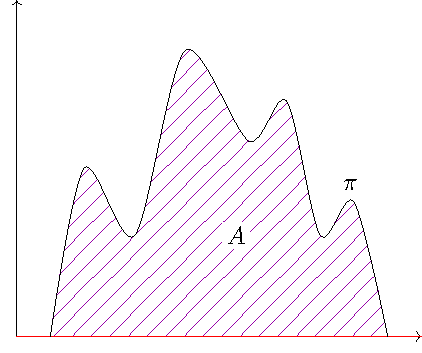
\includegraphics{../standalones/pdfs/areaunder}
\]
\begin{proof2}
    If (X,Y) is uniform on A we have $\pi_{X,Y}(x,y)\propto\mathbbm{1}_{0\leqslant y\leqslant\pi(x)}$ whose normalizing constant is
    \[
    \int_S\int_0^\infty\mathbbm{1}_{0\leqslant y\leqslant\pi(x)}\dif y \dif x =\ldots=1.\]
    Then the marginal of $X$ is
    \begin{align*}
        \int_0^\infty \pi_{X,Y}(x,y) \dif y&= \int_o^\infty \mathbbm{1}_{0\leqslant y\leqslant\pi(x)}\dif y\\
        &=\int_0^{\pi_X(x)}\dif y=\pi_X(x)
    \end{align*}
   \end{proof2}
   AR methods are based on this result. 
     How does this connect with Markov-Chain Monte-Carlo? The main idea is that we can use  a Markov Chain whose equilibrium distribution is a uniform on $A$, then discarded $Y$ and keep $X$. The target is \[\pi_{X|Y}(x,y) \alpha 1_{0 \leqslant y \leqslant \pi(x)} \] and we need to construct a Markov Chain that is ergodic with respect to this target.  We can think a Gibbs sampler that alternate the draws from the two condition:
    \begin{itemize}
        \item $Y'|X\sim \pi_{Y|X}(y|x)\propto\mathbbm{1}_{0\leqslant y\leqslant\pi(x)}$ ($x$ is fixed: this step sets the height of the \textit{vertical slice});
        \item $X'|Y\sim \pi_{X|Y}(x|y)\propto\mathbbm{1}_{0\leqslant y\leqslant\pi(x)}$ ($y$ is fixed: this step sets the length of the \textit{horizontal slice}).
    \end{itemize}
    \begin{figure}[H]
        \centering
        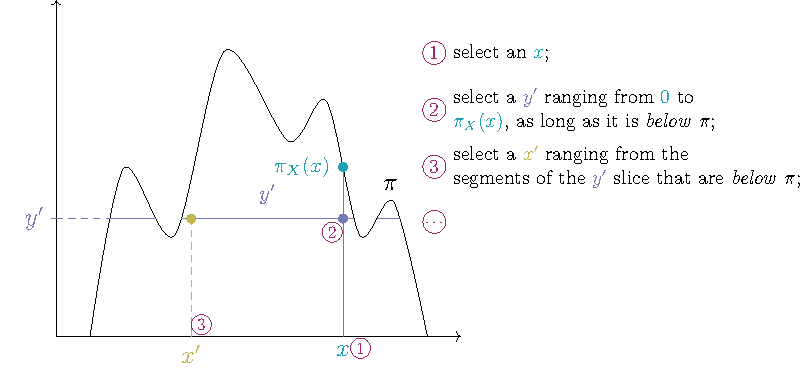
\includegraphics{../standalones/pdfs/slicesampler}
        \label{slicesampler}
    \end{figure}
So these are reversible step with respect to $\pi_{X,Y}$ and at equilibrium we have uniform sample on A: then using the lemma \ref{slizer}, $X$ is from $\pi_X$.
\begin{example}

$S=\mathbb{R}_+, \hspace{0.5 cm} \pi(x)=\frac{1}{2}e^{-\sqrt{x}}, x > 0$.
\begin{equation*}
    \pi^{-1}(y) = (\log2y)^2
\end{equation*}
so the slice sampler is 
\begin{itemize}
    \item $Y'|x \sim$ Unif $(0,\frac{1}{2}e^{-\sqrt{x}} )$
    \item $X'|y' \sim$ Unif $(0,(\log2y))^2$
\end{itemize}

$\pi(x) \propto e^{-\sqrt{x}}, x \in \mathbb{Z}_+$ unnormalized.
\begin{equation*}
    \pi^{-1}(y) = (\log(y))^2
\end{equation*}
\begin{itemize}
    \item $Y'|x \sim$ Unif $(0,e^{-\sqrt{x}} )$
    \item $X'|y' \sim$ Unif$(\{0,1,\ldots, \lfloor{(\log(y))^2 \rfloor}\})$ 
\end{itemize}
Remember that 
\begin{equation*}
    \left \lceil{x}\right \rceil =\max \{n \geqslant 0: n \leqslant x\}
\end{equation*}
If $\pi$ is d-dimensional, it is typically difficult to identify
\begin{equation*}
    A_y = \{x: y \leqslant \pi(x)\}
\end{equation*}
If we can write 
\begin{equation*}
    \pi(x) \propto \prod_{i = 1}^d \pi_i(x)
\end{equation*}
we can use $d$ auxiliary variables $y_1, \ldots, y_d$, so that 
\begin{equation*}
    \pi_i(x) = \int_0^{\pi_i(x)}\dif y_i = \int \mathbbm{1}_{0 \leqslant y_i \leqslant \pi_i(x)} \dif y_i
\end{equation*}
so the augmented target is 
\begin{equation*}
    \pi(x,y)=\pi(x_1, \ldots, x_d, y_1, \ldots, y_d) \propto \prod_{i = 1}^d \mathbbm{1}_{0 \leqslant y_i \leqslant \pi_i(x)} 
\end{equation*}
In the following graphs, the chain oscillates but stays stable around a certain level. Even if it seems not to converge, the oscillations are actually pretty stable and do not change throughout time. So the chain is convergent in the end.\\

Sometimes convergence of the MCMC is deceptive, as one run exhibits convergence but multiple runs reveal differently. \\
In these cases we can combine different strategies. \\
For example, if the transition matrices $P'$ and $P''$ both have invariant $\pi$, the convex linear combination 
\end{example}
\begin{equation*}
    P = w P' + (1-w) P'', \hspace{1 cm} w \in (0,1)
\end{equation*}
has invariant $\pi$ (exercise). \\
This is called a \enf{mixture transition}. This means that with probability w we use the matrix $P'$ and with compementary probability we use the matrix $P''$. \\
For example, one could choose
\begin{itemize}
    \item $P'$ as a RW-MH to explore locally
    \item $P''$ as an independent MH (that is, the proposal is independent on the current space: it is fixed) to explore globally 
\end{itemize}
so with w close to $1$, the chain once in a while takes a jump. This is useful to explore distribution with particularly low density areas that the chain will cross very seldom.\\
%take attention vibes
Example: local exploration and sometimes the chain takes a jump. 
More generally
\begin{equation*}
    P = \sum_{i = 1}^k w_i P:i, \hspace{1 cm} \sum_{i=1}^k w_i=1, \pi P_i = \pi
\end{equation*}
Another idea is to use a \enf{cycle transition}. 
\begin{equation*}
    P=P' P''    
\end{equation*}
which leaves $\pi$ invariant (exercise), but not reversible in general.\\
More generally, 
\begin{equation*}
    P=P_1P_2 \ldots P_k
\end{equation*}
For example, the multicomponent Gibbs sampler (with deterministic visits to coordinates).\\

%Esempio di un metodo con nome lungo
This method aims to update $k$ coordinates; when one of them is difficult to update it uses a Metropolis step to do it. \\
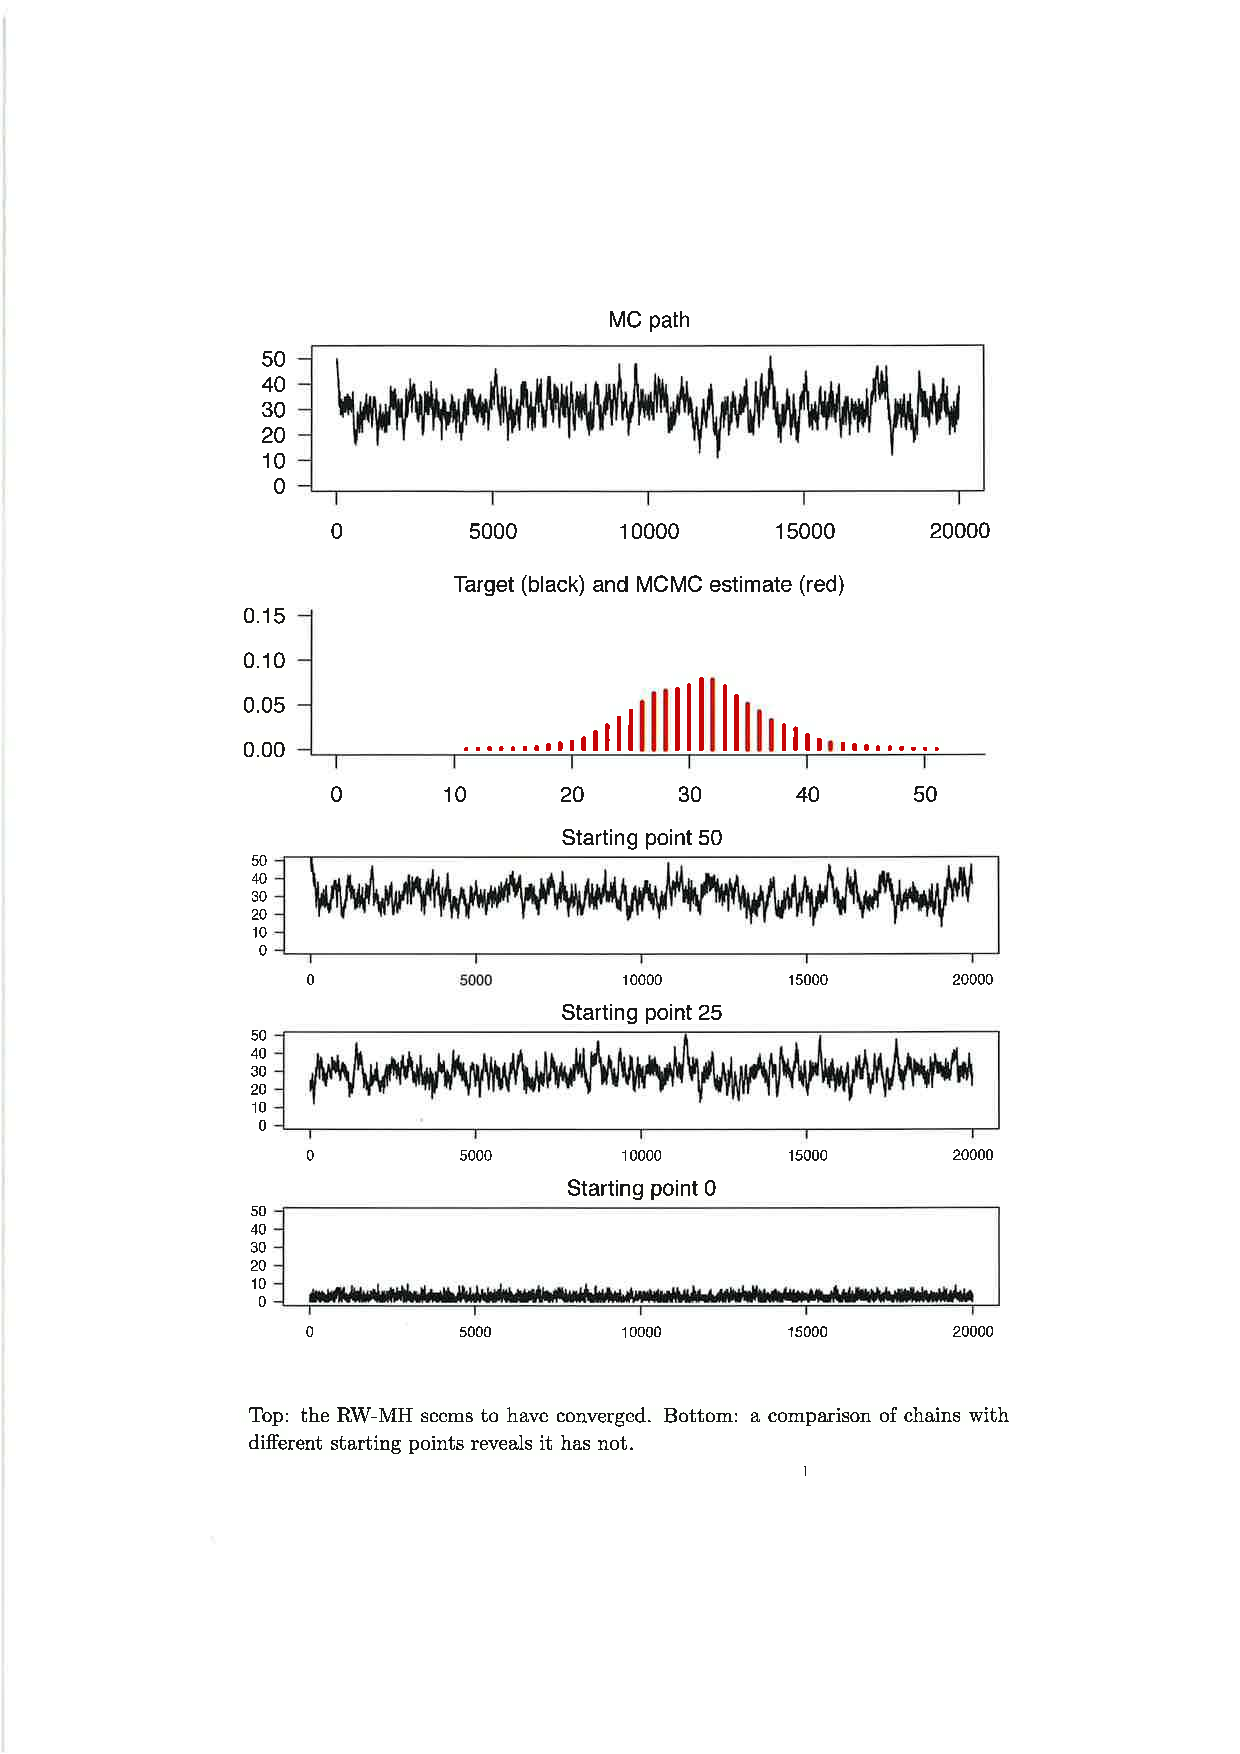
\includepdf[pages=-,pagecommand={}]{../external/fake conv}
Extensions and other methods:
\begin{itemize}
    \item \textbf{Reversible jump MCMC}: it moves among spaces of different dimensions.  
    \item \textbf{Langevin algorithms} or \textbf{gradient-based MCMC}: is it inspired by the Langevin diffusion
    \begin{equation*}
        dX_t = \frac{1}{2} \frac{d}{dX_t} \log\pi(X_t)dt + dB_t
    \end{equation*}
    It uses information on the gradient of $\pi$ to move towards regions of higher density.
\end{itemize}
There is a principle (Goldilocks's principle of MCMC): the variance of the steps has to be not too large, not too small.
\end{document}